\documentclass[a4paper]{article}
\usepackage[utf8]{inputenc}
\usepackage[spanish]{babel}
\usepackage{graphicx}
\graphicspath{{../BBDD/},{../Disenos/}}

\usepackage[colorlinks, backref]{hyperref}

\usepackage{color}
\definecolor{gray45}{gray}{.45}
\definecolor{gray97}{gray}{.97}
% \definecolor{gray7}{gray}{.7}
\usepackage{listings}
\lstset{
	language=sql,
	basicstyle=\small\ttfamily,
	numbers=left,
	numberstyle=\tiny,
	stepnumber=1,
	numbersep=5pt,
	backgroundcolor=\color{gray97},
	showspaces=false,
	showtabs=false,
	tabsize=8,
	breaklines=true,
	breakatwhitespace=false,
	showstringspaces=false,
% 	keywordstyle=\color{blue},
	commentstyle=\color{gray45},
	stringstyle=\color{red},
	showlines=false,
}

\title{Prueba LAMP Senior Developer}
\author{Miguel Ángel Ortiz Iglesias}
\date{\today}

\begin{document}
	\maketitle
	\tableofcontents
% 	\chapter{Introducción}
	\section{Introducción}
	El presente documento pretende ser uno de los requisitos que imponen en la prueba de capacidades  para desarrollador LAMP.
	
	El documento está dividido en una pequeña definición del problema, ver capitulo \ref{definicion}, un análisis  del problema, ver capitulo \ref{analisis}, la solución que se propone, ver capitulo \ref{solucion} y una serie de posibles mejoras, ver capitulo \ref{mejoras}.
% 	\chapter{Creación de un blog}\label{definicion}
	\section{Creación de un blog}\label{definicion}
	La prueba de capacidad consiste en la creación de un blog con detección de móvil (Marca/Modelo) que accede. El sistema tendrá una parte pública donde se pueden ver y crear los posts y una parte de admin donde se pueden censurar.
	
% 	\chapter{Análisis y diseño formal}\label{analisis}
	\section{Análisis y diseño formal}\label{analisis}
	En el presente capitulo se va a  explicar cual ha sido el resultado del análisis así como del diseño formal al que se ha llegado.
% 	\section{Análisis formal}
	\subsection{Análisis formal}
	Para poder ver los post que se han publicado es necesario tenerlos guardados en algún sitio, así como saber quien lo ha publicado, y si dicho post tiene una respuesta de alguien. Es por ello que se necesita una base de datos para poder acceder a dicha información.\newline
	También será necesario disponer de diferentes webs por las que navegar.\newline
	Cada usuario registrado dispone de una parte de administración para poder controlar y censurar los diferentes comentarios que consideré inapropiados y borrar en caso necesario algún post de los que ha publicado.
	
% 	\section{Diseño formal}
	\subsection{Diseño formal}
	El diseño se puede dividir en dos partes.
	\begin{enumerate}
		\item Diseño de la base de datos.
		\item Diseño de las webs en las que se compone la aplicación.
	\end{enumerate}
	
% 	\subsection{Diseño de la base de datos}
	\subsubsection{Diseño de la base de datos}
	La base de datos se ha realizado en UML, tal y como se puede observar en la figura \ref{modeloER}, y representan una primera versión de lo necesario para poder desarrollar la tarea. Cabe destacar que será necesario disponer de una segunda base de datos para poder guardar los datos de los usuarios así como de su contraseña de acceso.
	\begin{figure}[htb]
		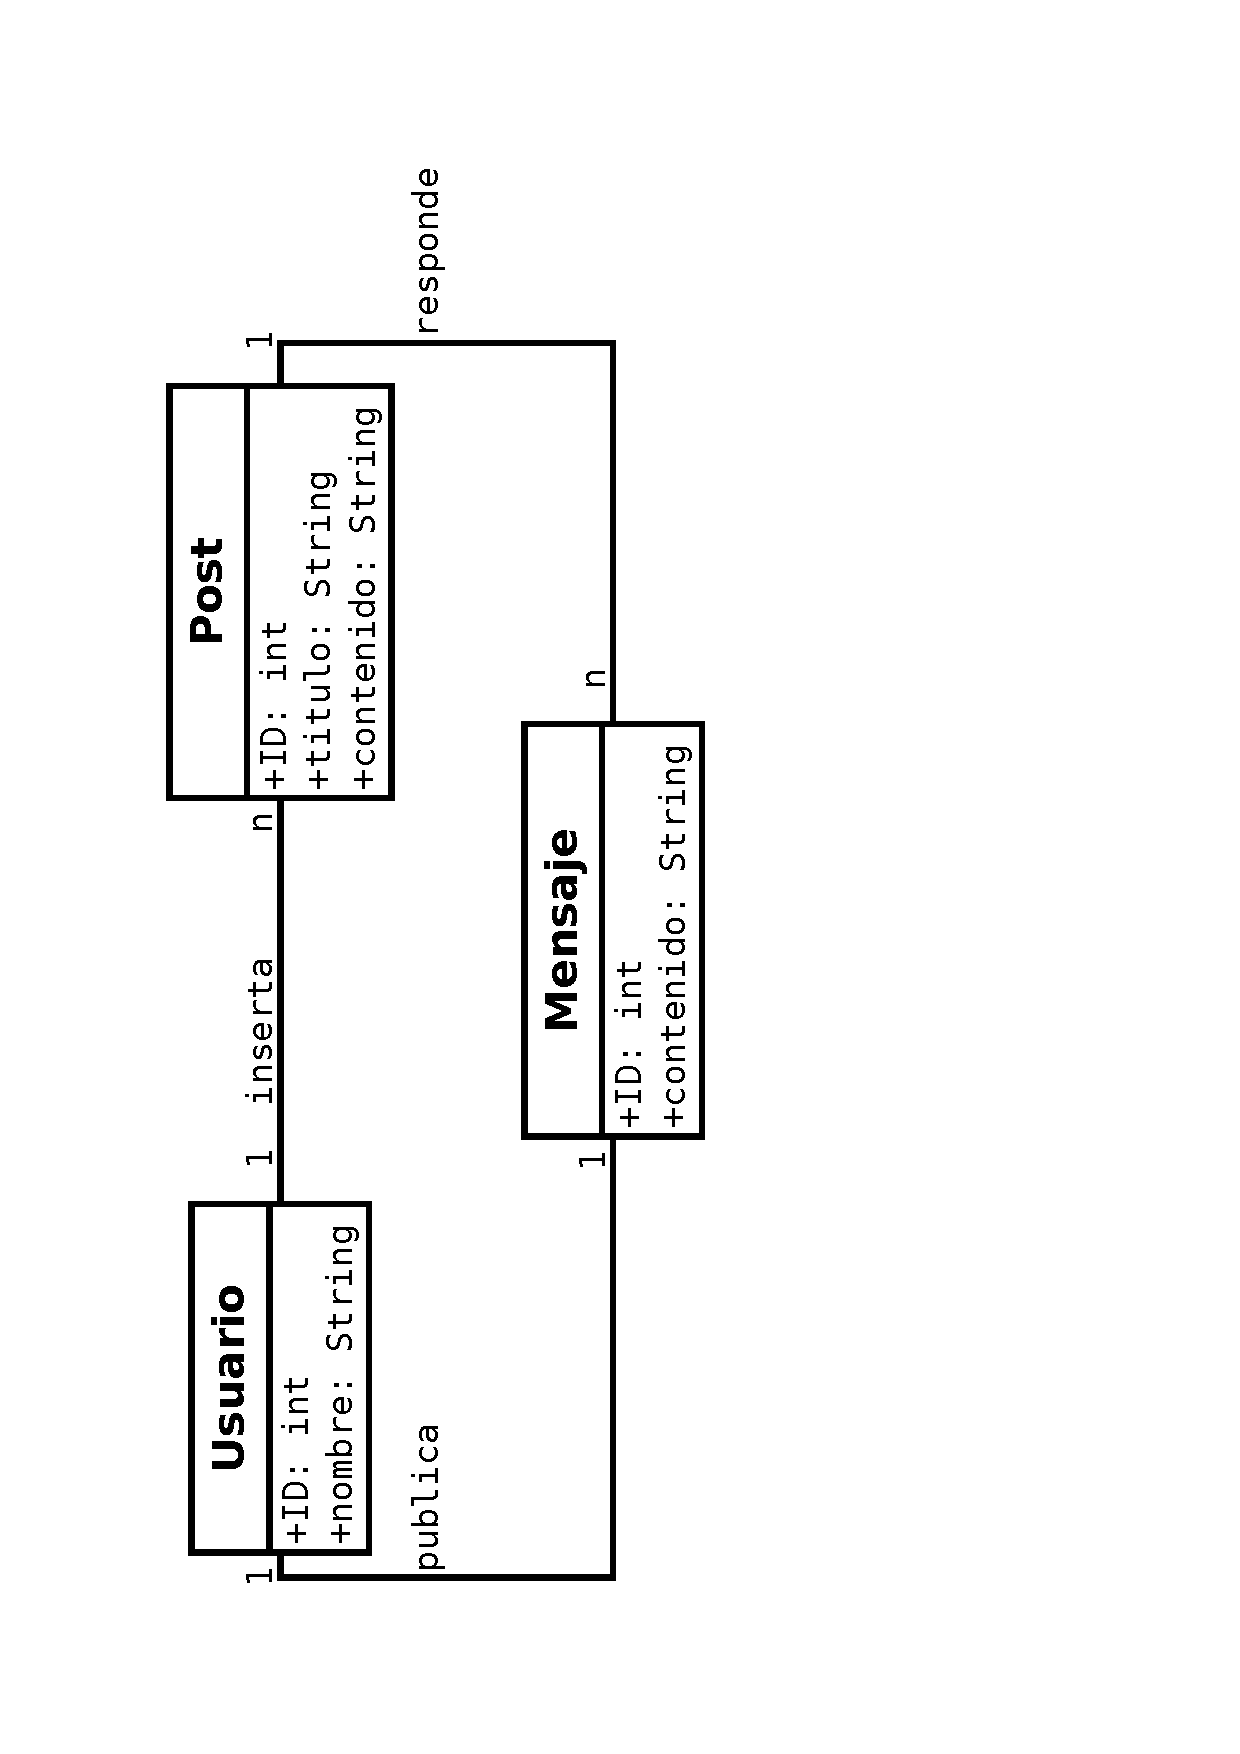
\includegraphics[keepaspectratio,width=\textwidth]{modeloER}
		\caption{Modelo UML}
		\label{modeloER}
	\end{figure}
	
% 	\subsection{Diseño de las webs}
	\subsubsection{Diseño de las webs}
	En las figuras \ref{home}, \ref{login}, \ref{post}, \ref{mensaje}, \ref{borrarPost}, \ref{borrarMensaje}, \ref{modificarDatos}, se pueden observar los diferentes diseños que se han planteado para cada una de las partes de la aplicación.
	\begin{figure}[htb]
		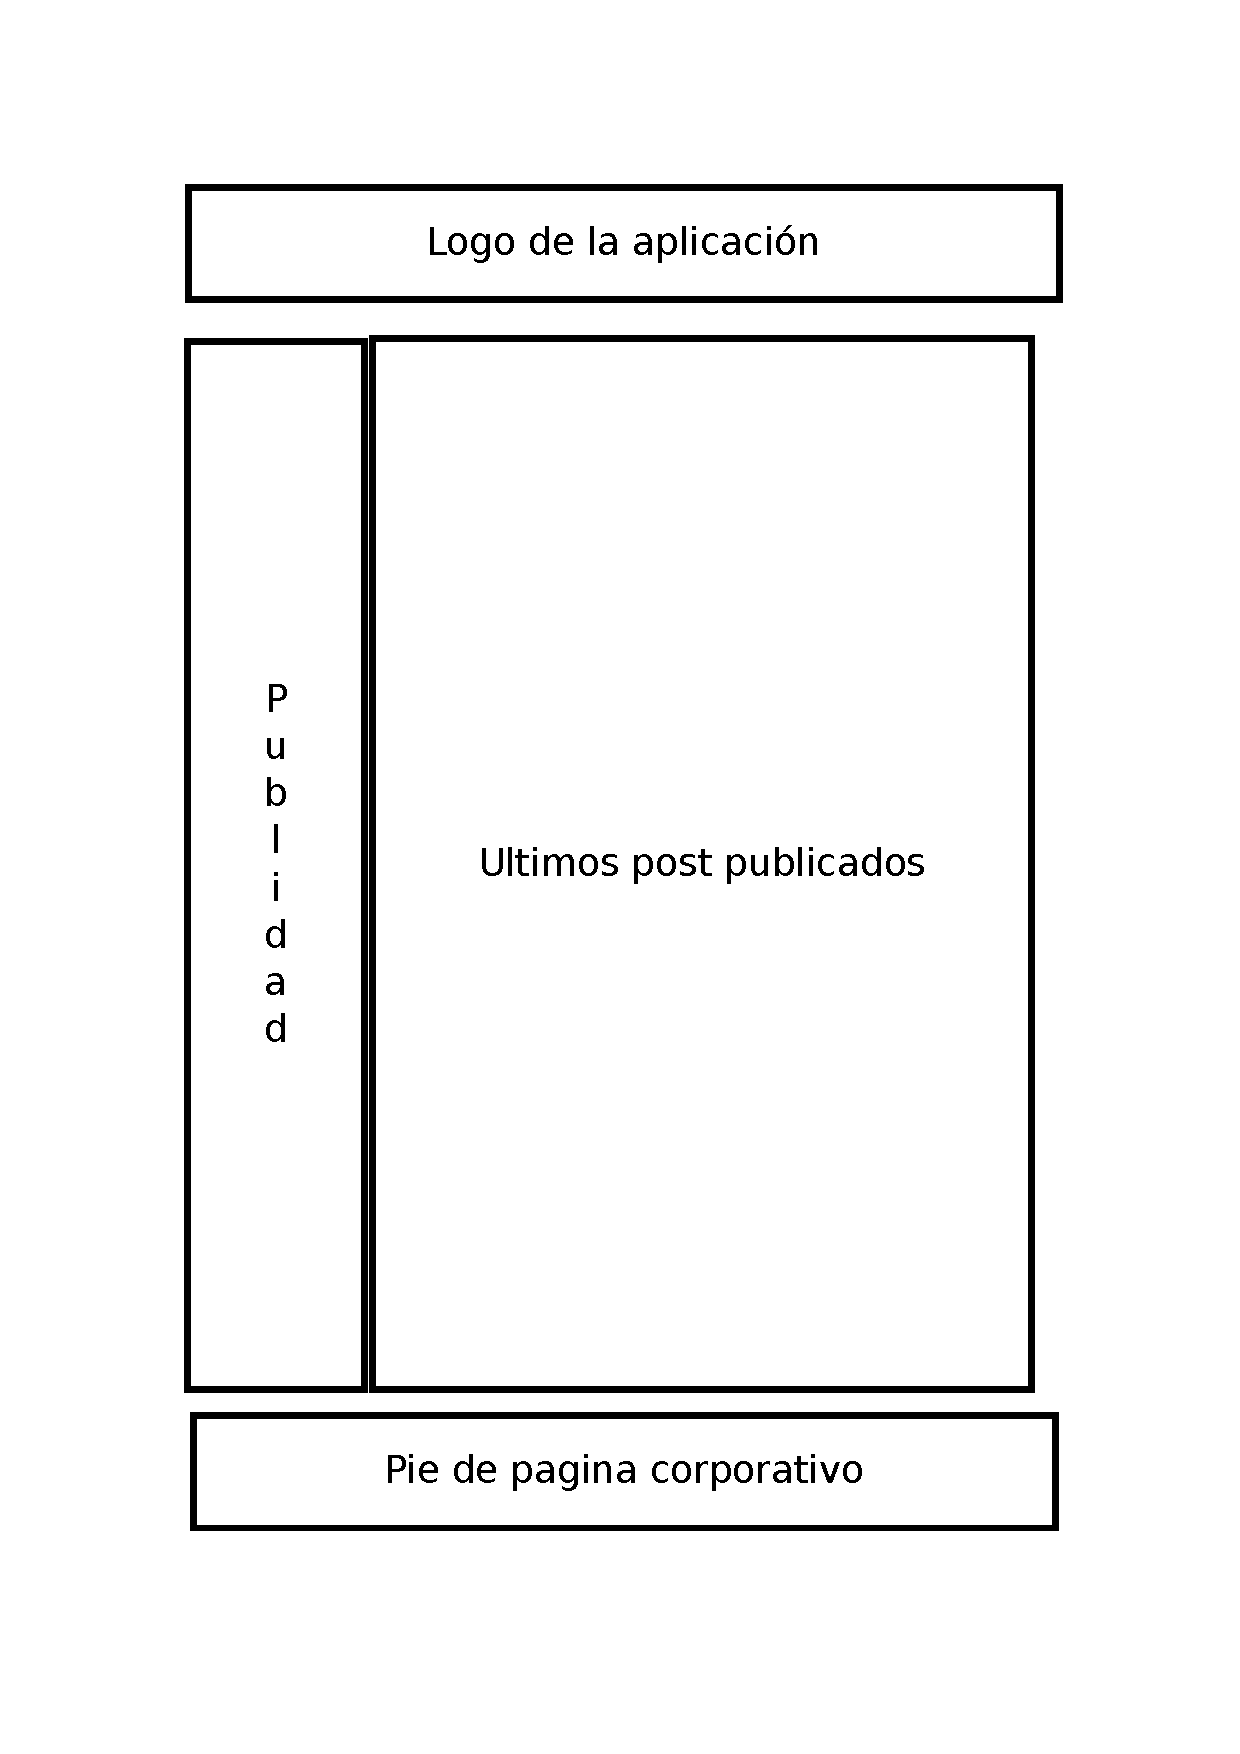
\includegraphics[keepaspectratio,width=\textwidth]{DisenoWebHome}
		\caption{Diseño de la home}
		\label{home}
	\end{figure}
	\begin{figure}[htb]
		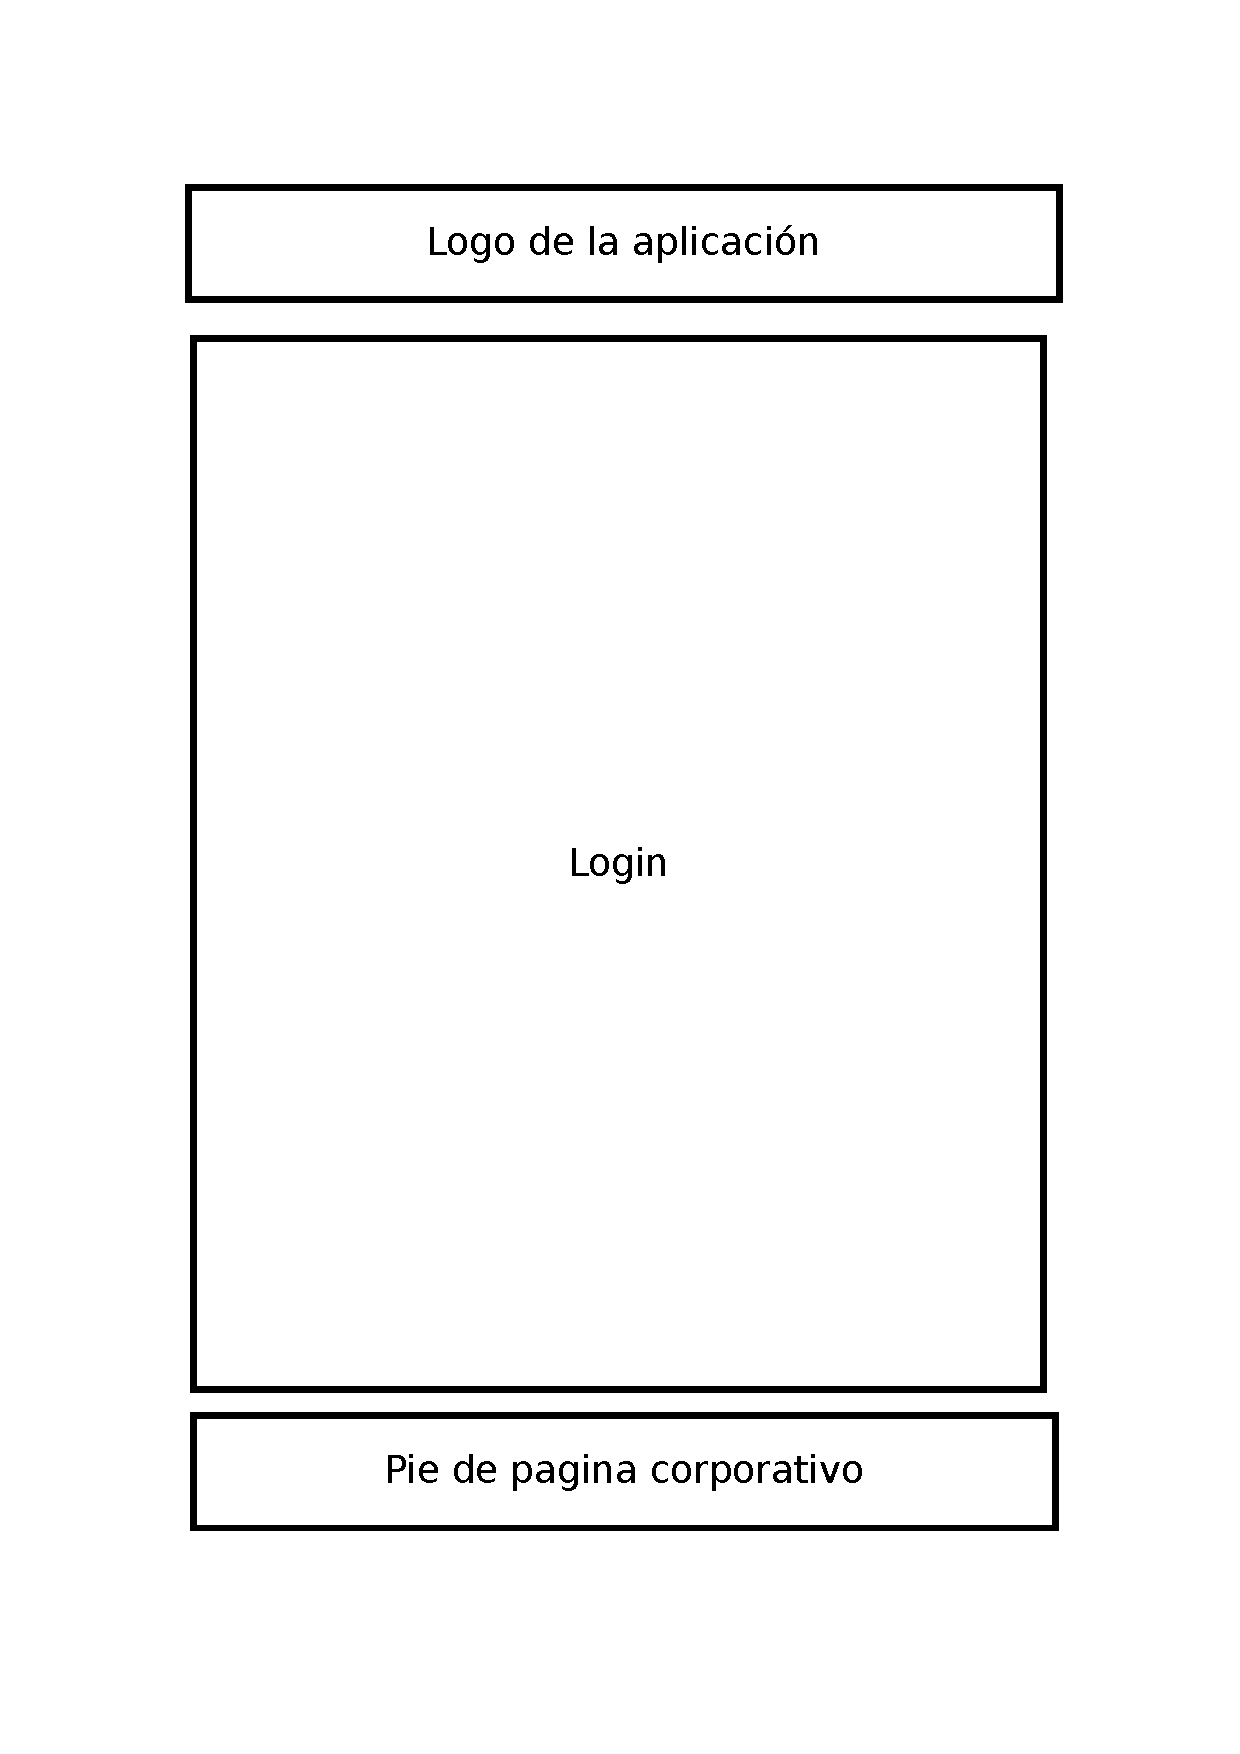
\includegraphics[keepaspectratio,width=\textwidth]{DisenoWebLogin}
		\caption{Diseño del login}
		\label{login}
	\end{figure}
	\begin{figure}[htb]
		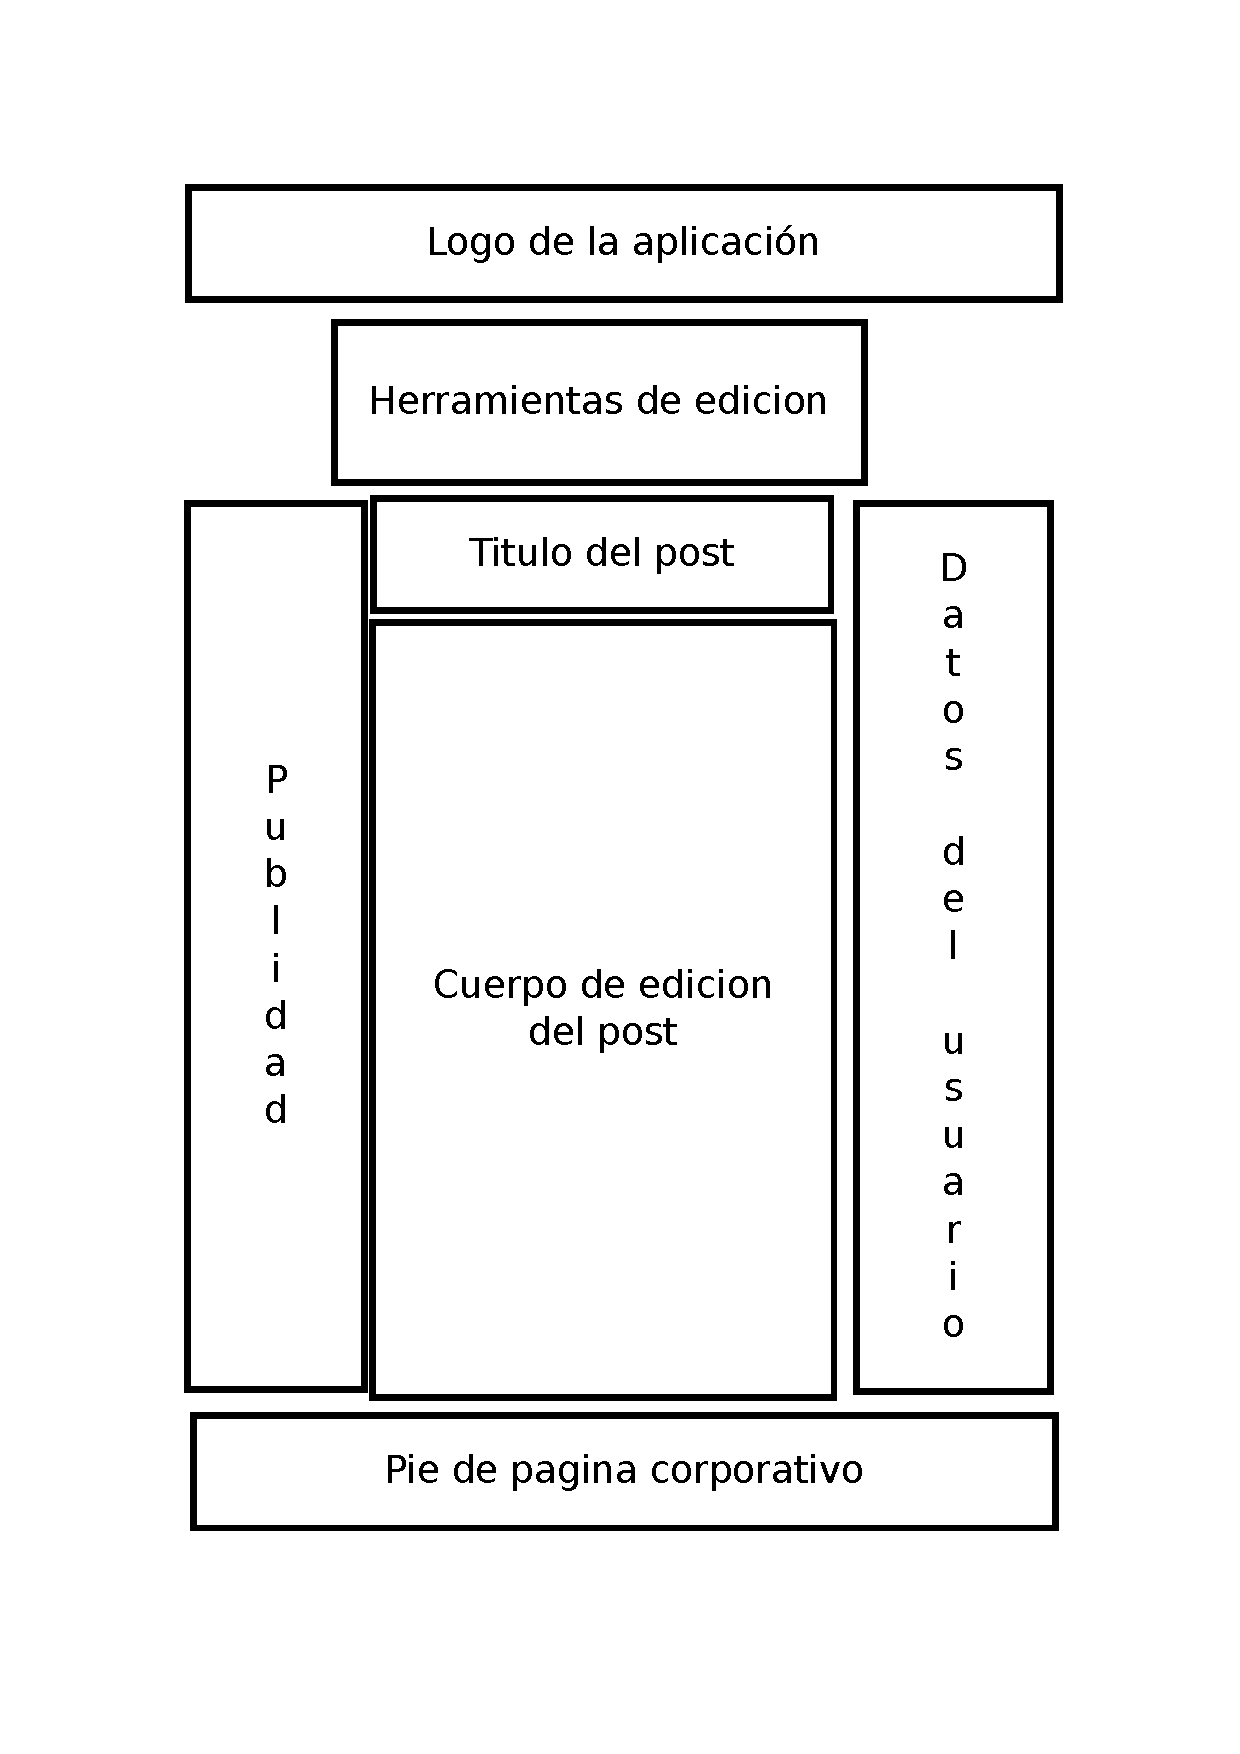
\includegraphics[keepaspectratio,width=\textwidth]{DisenoWebCreacionPosts}
		\caption{Diseño de la creación de posts}
		\label{post}
	\end{figure}
	\begin{figure}[htb]
		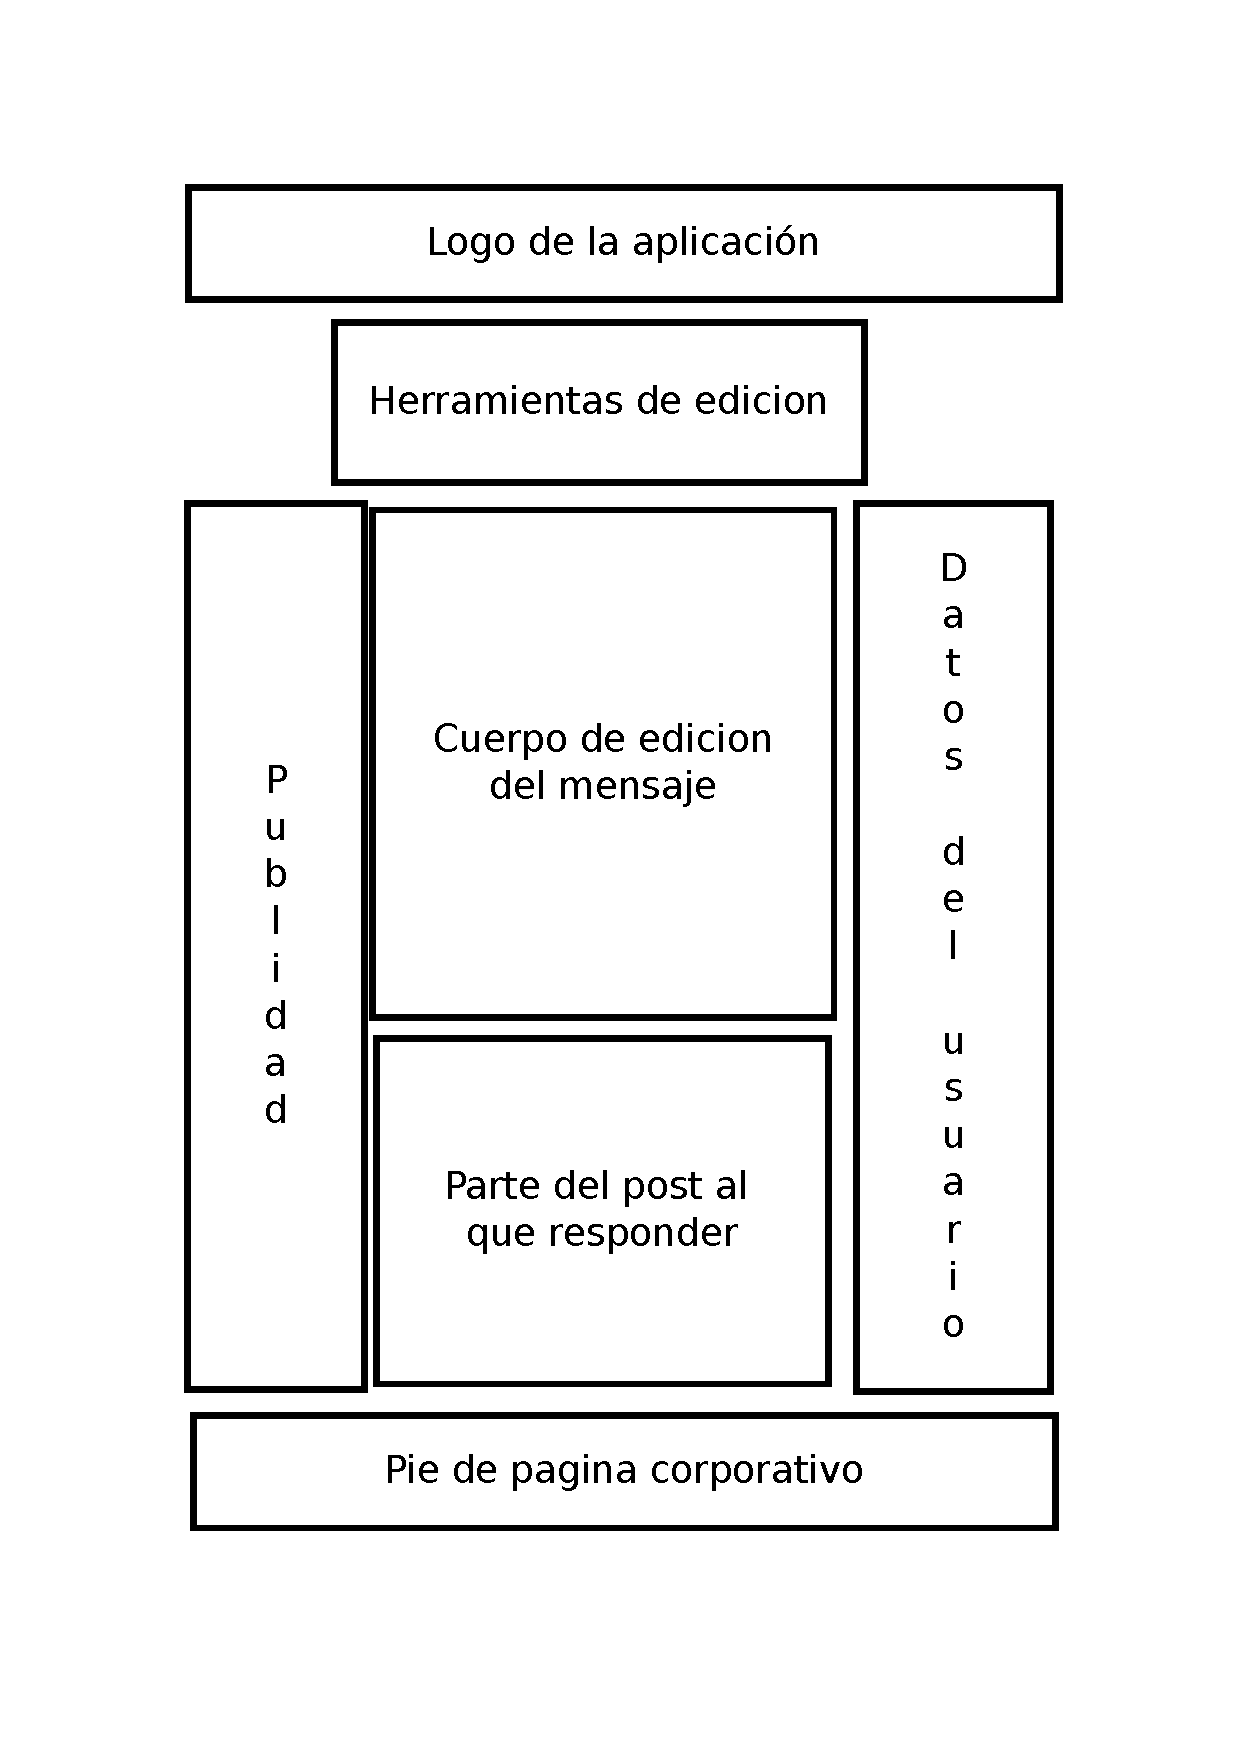
\includegraphics[keepaspectratio,width=\textwidth]{DisenoWebCreacionMensajes}
		\caption{Diseño de la creación de mensajes}
		\label{mensaje}
	\end{figure}
	\begin{figure}[htb]
		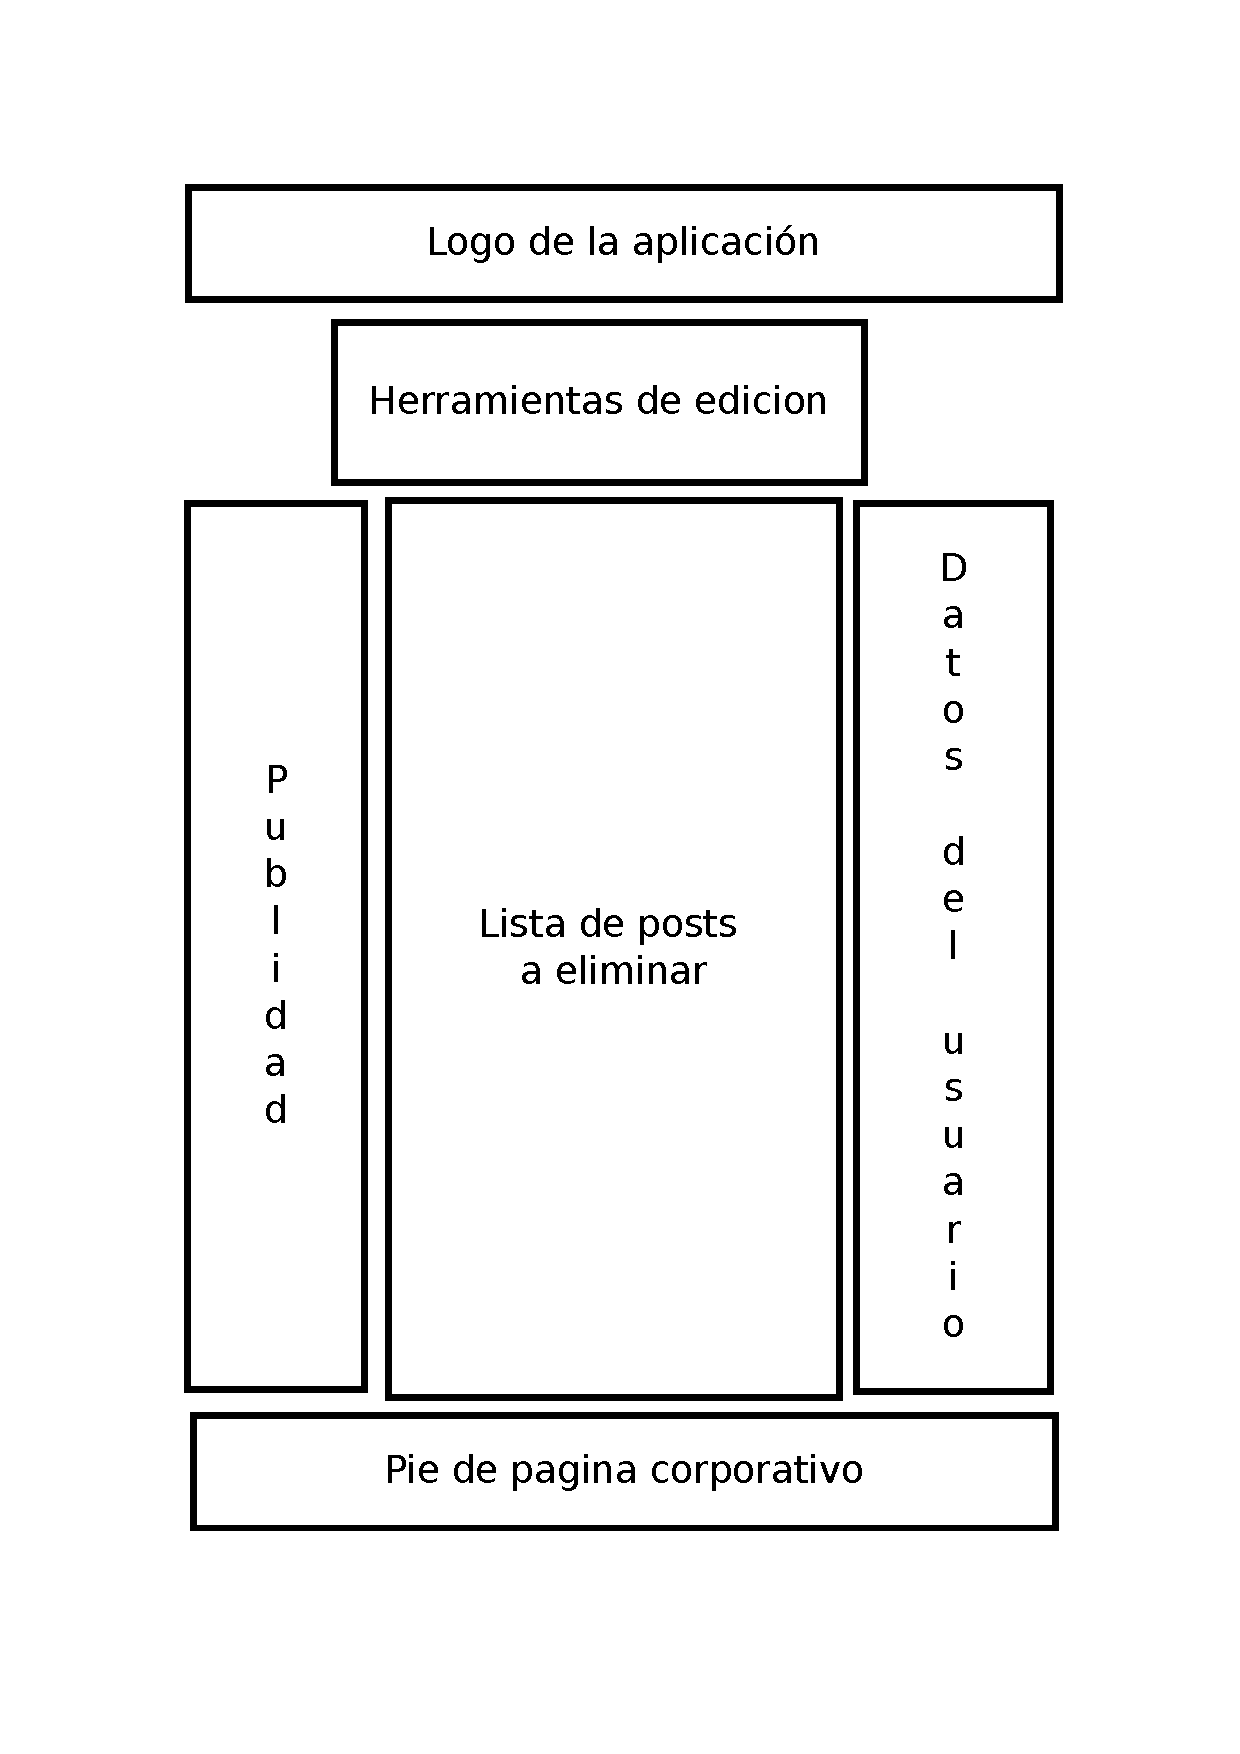
\includegraphics[keepaspectratio,width=\textwidth]{DisenoWebEliminacionPosts}
		\caption{}
		\label{borrarPost}
	\end{figure}
	\begin{figure}[htb]
		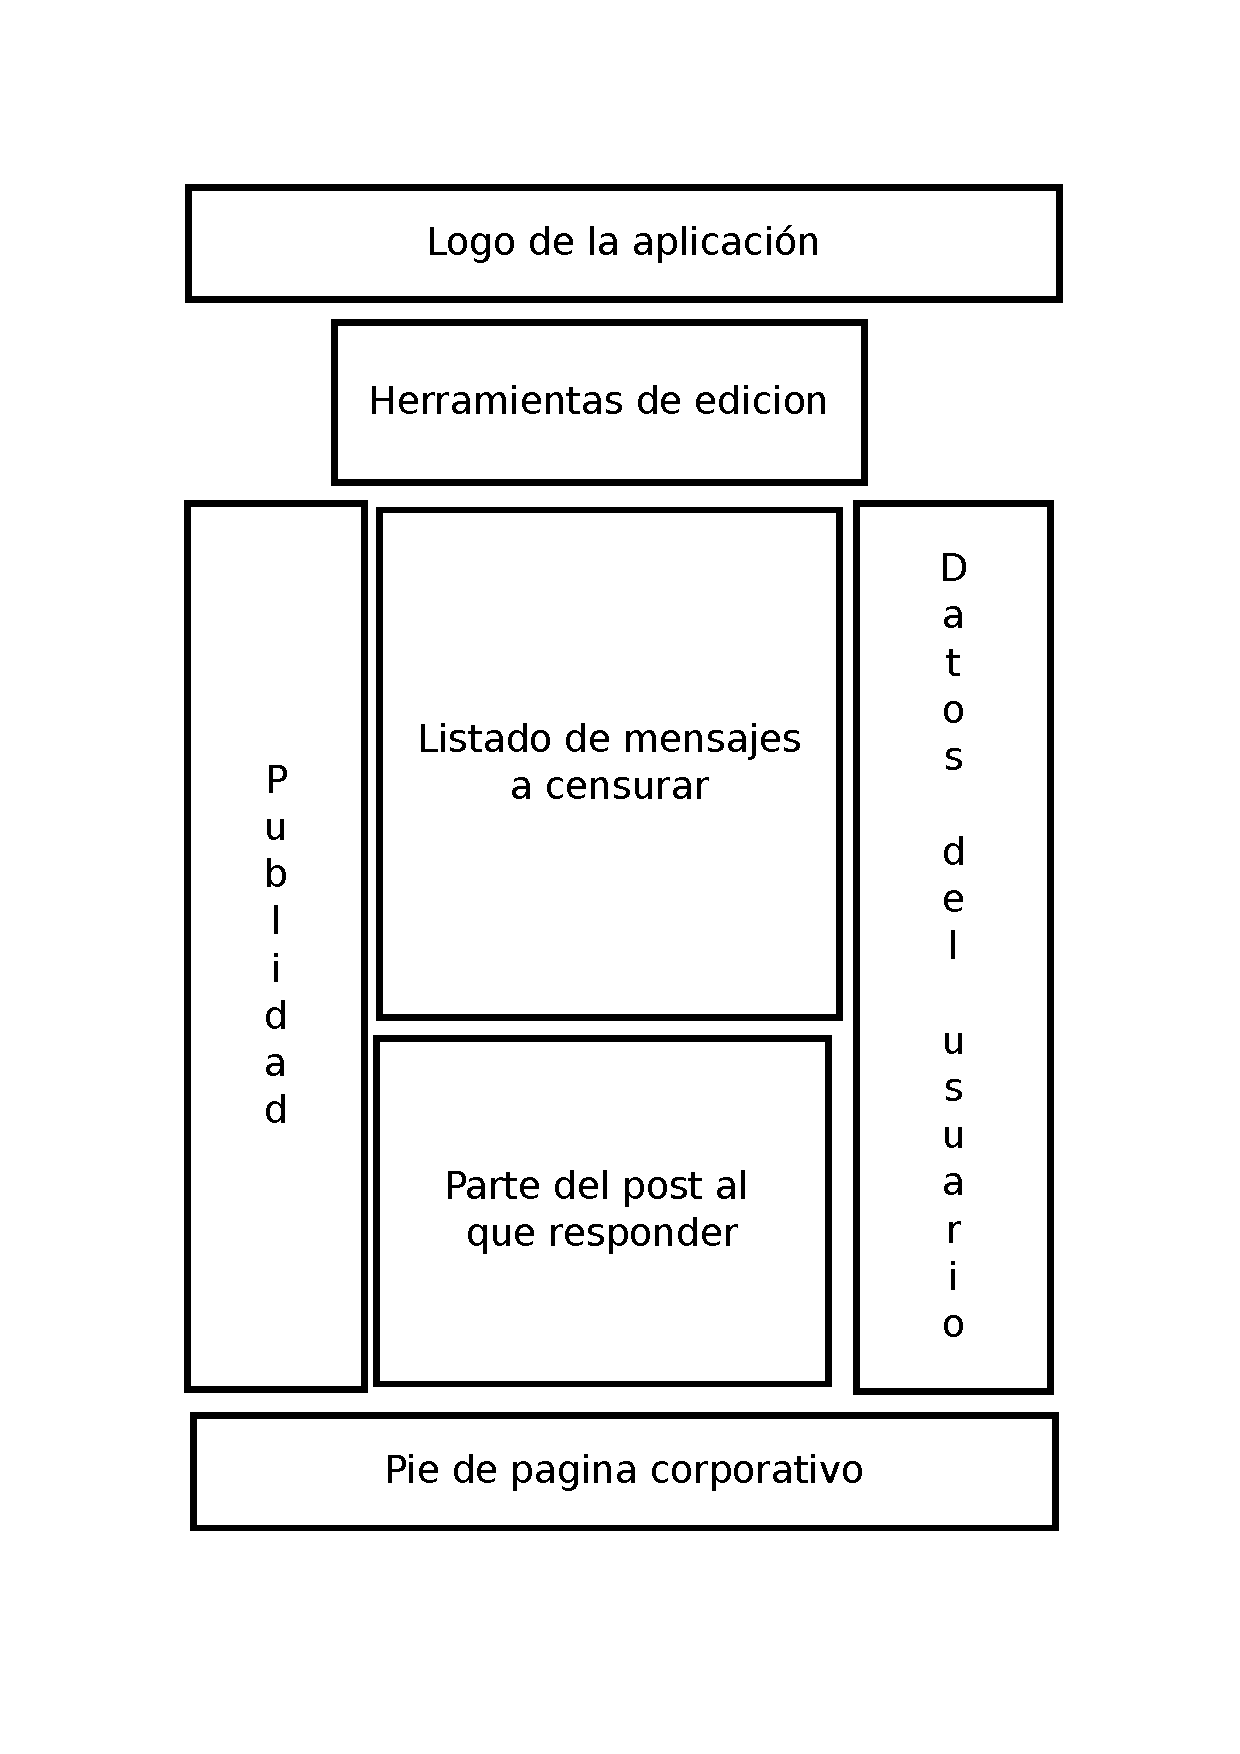
\includegraphics[keepaspectratio,width=\textwidth]{DisenoWebEliminacionMensajes}
		\caption{}
		\label{borrarMensaje}
	\end{figure}
	\begin{figure}[htb]
		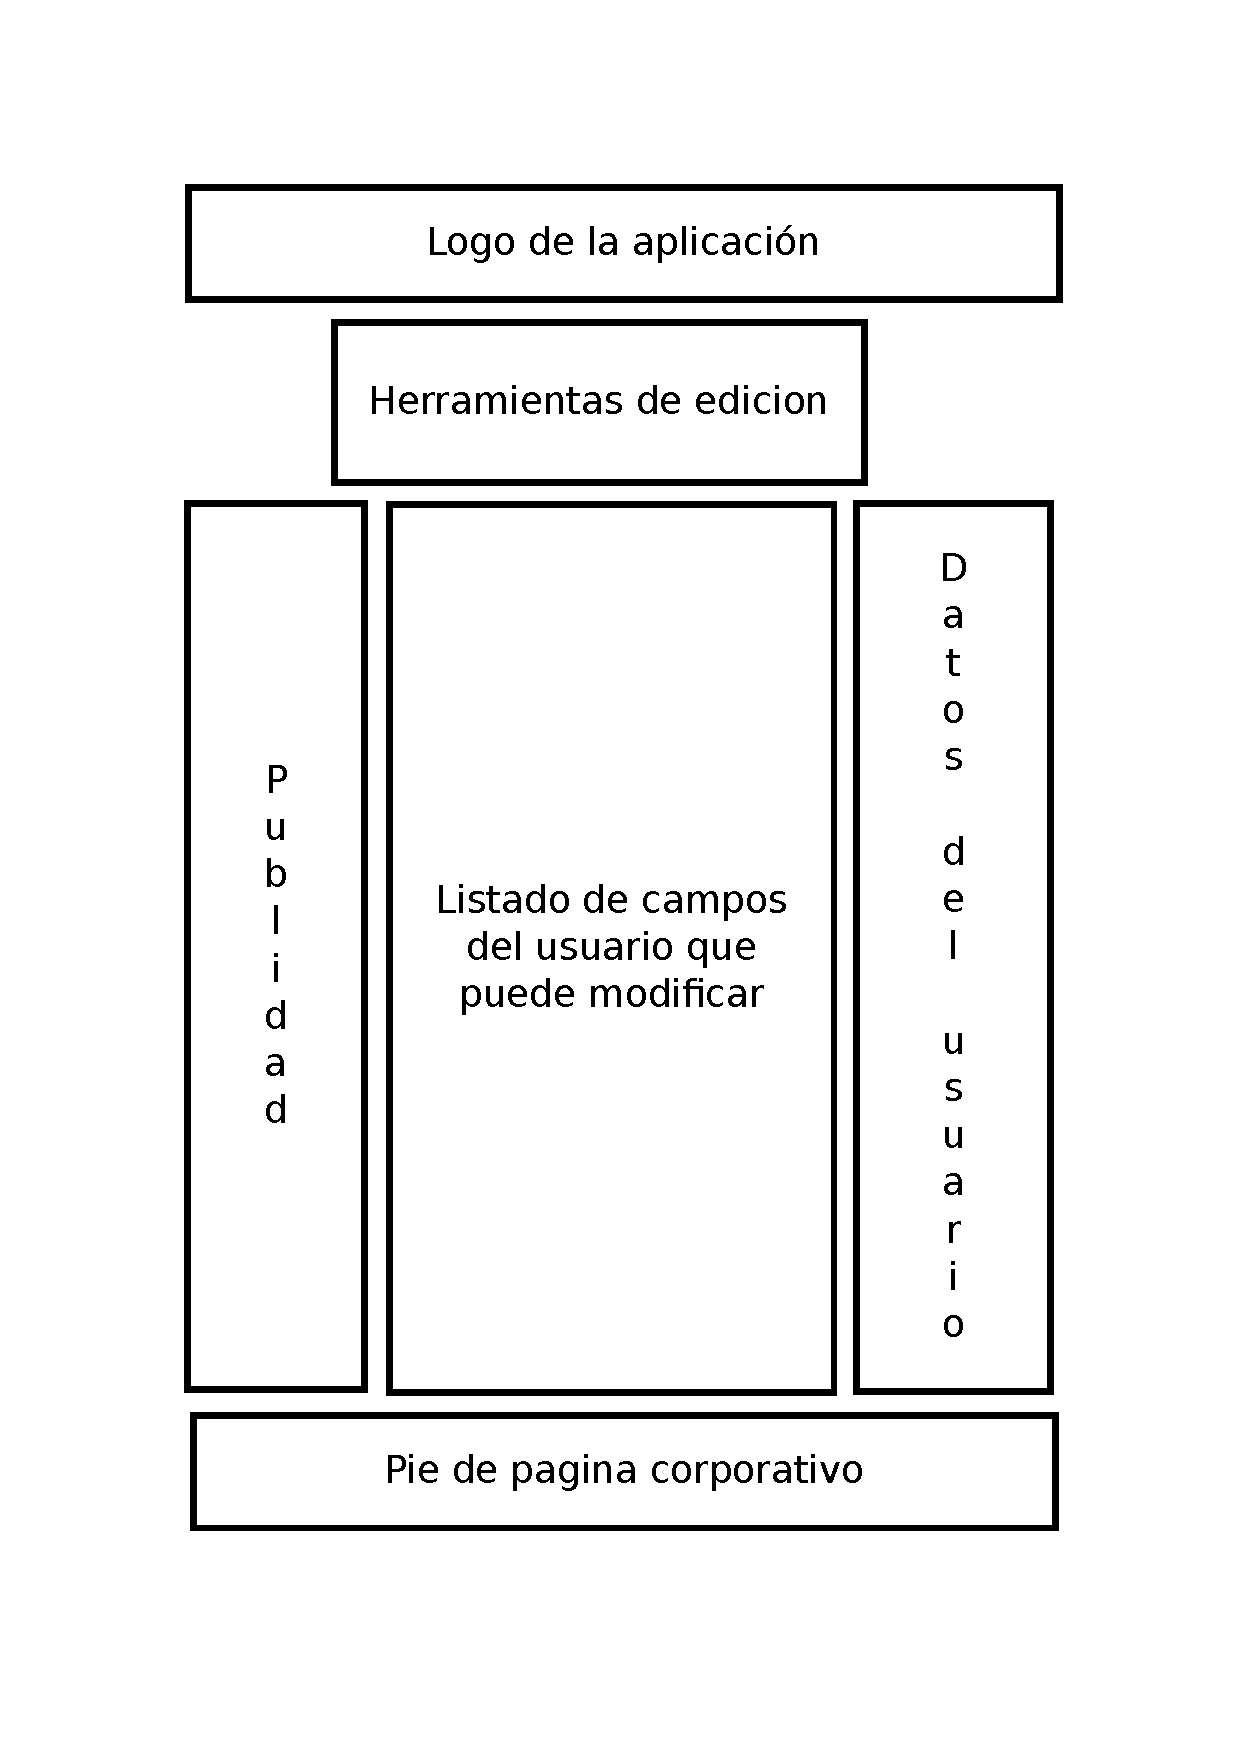
\includegraphics[keepaspectratio,width=\textwidth]{DisenoWebModificarDatos}
		\caption{}
		\label{modificarDatos}
	\end{figure}
	
% 	\chapter{Solución Propuesta}\label{solucion}
	\section{Solución Propuesta}\label{solucion}
% 	En el presente capítulo se van a mostrar los diversos diseños de las diferentes webs de la aplicación.
	La solución que se propone para por la creación de la base de datos en mysql, así como de una serie de consultas inserciones y actualizaciones de la misma.
	
	Para crear la base de datos se ha creado varios script.
	\subsection{Creación de la base de datos}
	\lstinputlisting{../BBDD/scriptCreacionBD.sql}
	\subsection{Creación del modelo de la base de datos}
	\lstinputlisting{../BBDD/scriptCreacionModeloBD.sql}
	
	\subsection{Ejemplos de consultas}
	
% 	Como ejemplo de consultas que mas se realizan se van a mostrar una serie de consultas.
	\lstinputlisting{../BBDD/ejemploConsultas.sql}
	\subsection{Ejemplos de inserciones}
	\lstinputlisting{../BBDD/ejemploInsercion.sql}
% 	\subsection{Ejemplos de actualizaciones}
% 	\lstinputlisting{}
	
% 	\chapter{Mejoras en la aplicación}\label{mejoras}
	\section{Mejoras en la aplicación}\label{mejoras}
% 	En el presente capítulo pretende ser un compendio de 
% 	Existen toda una serie de mejoras que se tienen que estudiar para ver si son factibles instalarlas.
	
	\begin{itemize}
		\item Añadir una base de datos con los datos y las contraseñas de los usuarios.
	\end{itemize}
	
	
% 	\section{Precisión}
% 	Usar los conceptos y/o términos, definir los conceptos y explicarlos la primera vez que salen, definir los acrónimos.
% 	\section{Claridad}
% 	Ordenar las cosas, de lo general a lo particular. No usar conceptos que no ha sido definidos
% 	\chapter{Solución Propuesta}
% 	Planificar y hacer esquemas.
% 	\section{Introducción}
% 	\section{Antecedentes}
% 	\section{Planteamientos}
% 	\section{Partes}
% 	\section{Resultados}
% 	\section{Conclusiones}
% 	\chapter{Problemas encontrados}
% 	
% 	\chapter{Conclusiones}
% 	
% 	\chapter{Sugerencias}
% 	
% 	\chapter{Bibliografía}
% 	Usar las referencias bibliográficas que ofrece \LaTeX.
% 	\chapter{Apéndices}
% 	
% 	\section{Código Fuente}
% 	
% 	\section{Manual de Usuario}
% 	
% 	\section{Tabla de Figuras}
	%\tableoffigures
	
\end{document}